\documentclass[journal]{IEEEtran}
\renewcommand{\IEEEkeywordsname}{Keywords}

\usepackage[italian]{babel}
\usepackage[utf8]{inputenc}
\usepackage[T1]{fontenc}

\setlength{\marginparwidth}{2cm}
\usepackage[italian, textsize=small, textwidth=2cm]{todonotes}

\usepackage{hyperref}
\usepackage{url}
\usepackage{tikz}
\usetikzlibrary{shapes.geometric, arrows}
\usepackage[dvipsnames]{xcolor}
\usepackage{listings}
\usepackage{caption}
\renewcommand{\lstlistingname}{Codice}

\newcommand{\bigo}[1]{\ensuremath{O\left({#1}\right)}}
\usepackage{booktabs}
\usepackage{mathtools}
\DeclarePairedDelimiter\bra{\langle}{\rvert}
\DeclarePairedDelimiter\ket{\lvert}{\rangle}
\DeclarePairedDelimiterX\braket[2]{\langle}{\rangle}{#1\,\delimsize\vert\,\mathopen{}#2}
\usepackage{amsmath, amssymb}
\usepackage{algorithm}
\usepackage{algpseudocode}
\floatname{algorithm}{Algoritmo}

\usepackage{graphicx}
\graphicspath{ {./img/} }

\usepackage{amsthm}

\usepackage{listings}
\usepackage{xcolor}
% Configuration for pseudocode
\usepackage{listings,newtxtt,xcolor}
% Define custom colors
\definecolor{keywordcolor}{rgb}{0.1, 0.1, 0.75}  % Blue for keywords
\definecolor{stringcolor}{rgb}{0.1, 0.5, 0.1}    % Green for strings
\definecolor{commentcolor}{rgb}{0.5, 0.5, 0.5}   % Gray for comments
\definecolor{bgcolor}{rgb}{0.95, 0.95, 0.92}     % Light gray background

% Configure lstset for Python
\lstset{
    language=Matlab,                    % Set the language to Python
    backgroundcolor=\color{bgcolor},   % Background color for code
    basicstyle=\ttfamily\footnotesize, 
	keywordstyle=\color{keywordcolor}\bfseries, % Keywords in bold blue
    stringstyle=\color{stringcolor},   % Strings in green
    commentstyle=\color{commentcolor}\itshape, % Comments in italic gray
    identifierstyle=,                  % Default identifier style
    showstringspaces=false,            % Don't show spaces in strings
    numbers=left,                      % Line numbers on the left
    numberstyle=\tiny\color{commentcolor}, % Line number style
    numbersep=5pt, % Spaziatura dei numeri di riga
    %  frame=single, % Cornice intorno al blocco di codice
    % framerule=0.1pt,
    linewidth=0.98\columnwidth,
    stepnumber=1,                      % Line numbers increment by 1
    tabsize=4,                         % Tab size
    breaklines=true,                   % Automatically break long lines
    breakatwhitespace=true,            % Break lines only at whitespace
    frame=single,                      % Draw a box around the code
    captionpos=b,                      % Caption position: b for bottom
    escapeinside={(*@}{@*)},           % Escape to LaTeX between (*@ and @*)
}

\theoremstyle{definition}
\newtheorem{definition}{Definizione}

\begin{document}

\title{Introduzione alla teoria della percolazione}

\author{\IEEEauthorblockN{Leonardo Ongari}
\IEEEauthorblockA{\textit{Università degli studi di Parma} \\
Cremona, Italia\\
leonardo.ongari@studenti.unipr.it}\\
}

\maketitle

\begin{abstract}
	La teoria della percolazione si occupa di sviluppare modelli matematici per descrivere il 
	fenomeno fisico della percolazione, caratterizzato dallo scorrimento di un \textit{fluido} 
	all'interno di un \textit{mezzo}. In questa relazione vengono mostrate le caratteristiche
	principali dei modelli, le nozioni teoriche associate ed alcune analisi sugli algoritmi 
	utilizzabili per effettuare simulazioni consistenti.   
\end{abstract}

\begin{IEEEkeywords}
Percolazione, Modelli, Simulazioni
\end{IEEEkeywords}

\section{Introduzione}

La teoria della percolazione nasce con l'obiettivo di ottenere un modello matematico 
per descrivere il fenomeno fisico della percolazione. Questo fenomeno descrive lo scorrimento 
di un fluido all'interno di un materiale tipicamente poroso. È importante specificare 
che il significato del termine ``percolazione'' può riferirsi a diversi contesti, 
a seconda del campo in cui si sta operando. Alcuni esempi sono: 
\begin{itemize}
    \item un soluto che diffonde attraverso un solvente;
    \item elettroni che migrano attraverso un reticolo atomico;
    \item molecole che penetrano un solido poroso;
    \item una malattia che infetta una comunità.
\end{itemize}
La formalizzazione matematica del problema ha reso possibile la creazione 
di un \textit{modello}. Un punto chiave molto importante di un modello 
è il concetto di \textit{astrazione}, caratteristica che permette di
operare senza considerare alcune variabili dipendenti dal contesto \cite{broadbent}.
\section{Background}
\label{sec:background}

Un metodo efficace per l'astrazione del concetto consiste 
in una rappresentazione tramite un reticolo, in inglese ``lattice''.

% \begin{definition}[Reticolo]
%     Un reticolo è un insieme di punti (siti), ciascuno in grado di identificare un 
%     ordine locale per il riconoscimento dei primi vicini.
%     I siti sono collegati tra di loro tramite degli archi (legami), che 
%     possono esistere solo tra due primi vicini.
% \end{definition}

\begin{definition}[Reticolo]
    Un reticolo $L$ di dimensione $n$ è una coppia $\langle S, B \rangle$, dove:
    \begin{itemize}
        \item $S = \left\{ s_i : i \in \mathbb{N} , \, 0 \leq i < n \right\}$ è l'insieme dei siti;
        \item $B = \left\{ (s_i, s_j) \in S^2 \, : \text{$s_i$ e $s_j$ siano primi vicini} \right\}$ è 
        
        l'insieme dei legami.
    \end{itemize}
\end{definition}
Due siti possono essere considerati primi vicini se, secondo l'ordinamento locale dei siti, hanno 
distanza uguale a 1.
In un reticolo in cui vale questa relazione è possibile descrivere due tipi di percolazione: 
percolazione di sito e percolazione di legame.
% \begin{itemize}
%     \item percolazione di legame;
%     \item percolazione di sito.
% \end{itemize}

\begin{figure}
    \centering
    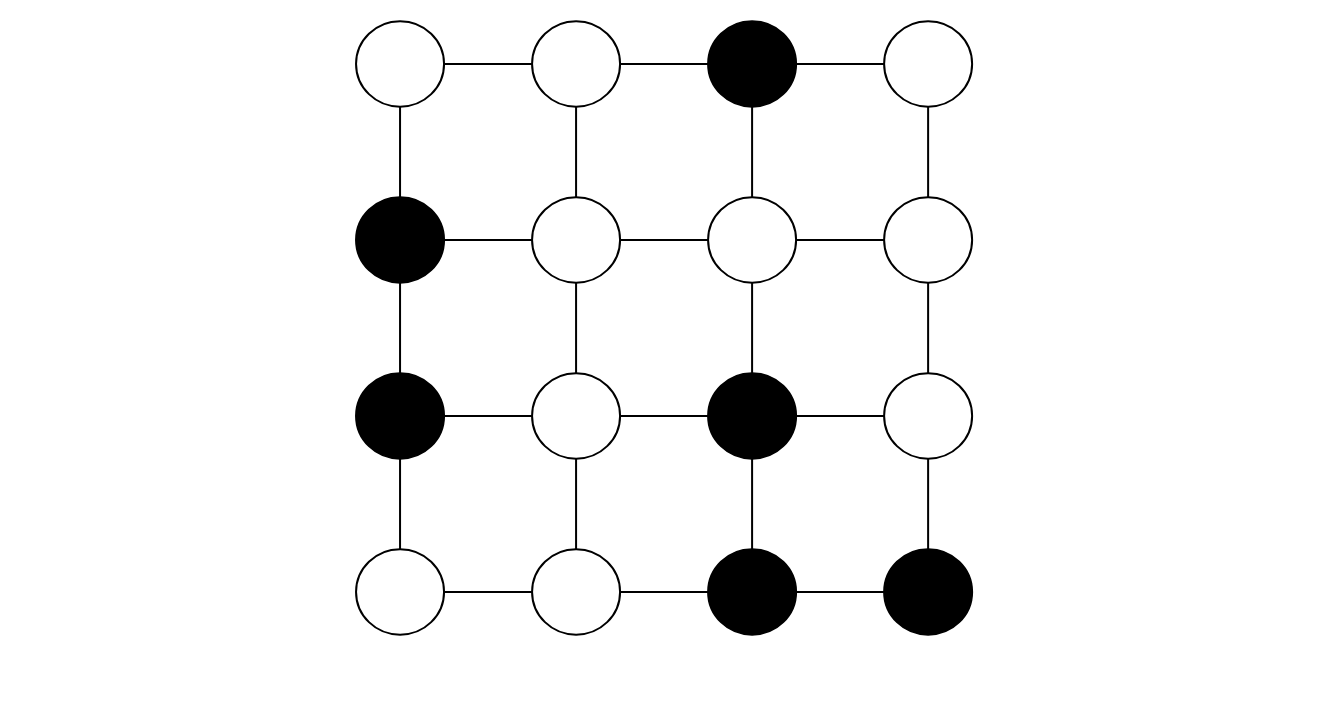
\includegraphics[width=0.4\textwidth]{2D-lattice}
    \caption{Esempio di reticolo quadrato bidimensionale}
    \label{fig:ex-lattice}
\end{figure}

\subsection*{Percolazione di legame}
È la prima versione del modello fornita da Broadbent e Hammersley \cite{broadbent}.
Ogni legame ha probabilità $p$ di essere ``aperto'', quindi
probabilità $1-p$ di essere ``chiuso''. Se due siti formano un legame aperto, vi è una
connessione diretta tra i due. Al contrario, un legame chiuso elimina la connessione.
In questa versione, ``avviene percolazione'' se esiste un percorso (insieme di connessioni dirette) 
che attraversa l'intero reticolo. La percolazione può verificarsi 
sia in verticale (alto-basso) sia in orizzontale (sinistra-destra).

\subsection*{Percolazione di sito}
In questo modello ogni sito ha una probabilità $p$ di essere occupato, di conseguenza
probabilità $1-p$ di essere vuoto. In figura \ref{fig:ex-lattice} viene mostrato un 
reticolo bidimensionale quadrato con nodi occupati (neri) e vuoti (bianchi). Questo è 
il modello che verrà utilizzato per lo studio dell'argomento e dei vari algoritmi e verrà
approfondito in dettaglio nella sezione \ref{sec:implementazione}.

\subsection*{Soglia di percolazione}
I due modelli appena introdotti rappresentano soluzioni valide per lo studio 
del fenomeno. Nonostante la somiglianza, vi sono differenze concettuali che si 
riflettono anche nel calcolo di alcuni valori caratteristici \cite{weisstein-bond,weisstein-site,weisstein-threshold}.

\begin{definition}[Soglia di percolazione]
    Sia $L$ un reticolo di dimensione infinita\footnote{Con il termine ``infinito'' 
    si fa riferimento all'estensione intuitiva delle varie proprietà della struttura,
    come avviene in matematica per il concetto di \textit{limite all'infinito}.}. 
    Sia $p$ la probabilità di occupazione di un sito o di apertura 
    di un legame, a seconda del modello scelto. 
    Sia $p$ uguale per ogni elemento del reticolo.
    La soglia di percolazione per $L$ è definita come la 
    probabilità $p_c$ tale per cui:
    \begin{itemize}
        \item se $p > p_c$, allora vi è percolazione;
        \item se $p < p_c$, allora non vi è percolazione.
    \end{itemize}
\end{definition}

\begin{figure}
    \centering
    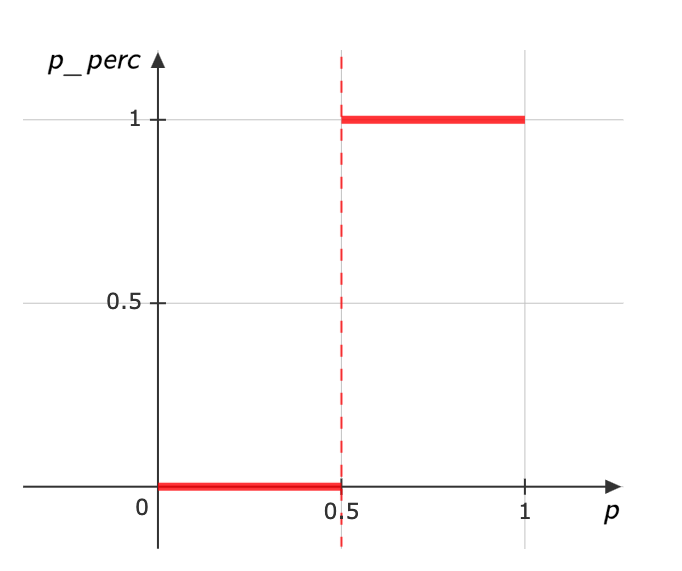
\includegraphics[width=0.4\textwidth]{threshold.png}
    \caption{Grafico relativo alla soglia di percolazione ($p_c=0.5$)}
    \label{fig:threshold}
\end{figure}

È possibile visualizzare il concetto di soglia nel grafico mostrato in 
figura \ref{fig:threshold}, in cui l'asse delle ascisse è associato alla 
probabilità $p$, mentre l'asse delle ordinate è associato alla probabilità
che avvenga percolazione $p_{perc}$.

Nei casi reali, ovvero per reticoli di taglia finita, non è possibile stabilire
un'affermazione così forte. 
Ciò che è possibile preservare dalla definizione 
è che esiste un \textbf{punto critico} $p_c$ relativo alla probabilità $p$, oltre 
al quale è più probabile che avvenga percolazione e, al contrario, al di sotto
del quale è meno probabile che questo si verifichi.

\begin{table}[ht!]
    \centering
    \begin{tabular}{lcc}
    \toprule
    \textbf{Lattice} & \textbf{\(p_c\) (Site)} & \textbf{\(p_c\) (Bond)} \\
    \midrule
    Cubic (body-centered) & 0.246    & 0.1803    \\
    Cubic (face-centered) & 0.198    & 0.119     \\
    Cubic (simple)        & 0.3116   & 0.2488    \\
    Diamond               & 0.43     & 0.388     \\
    Honeycomb             & 0.6962   & 0.65271*  \\
    4-Hypercubic          & 0.197    & 0.1601    \\
    5-Hypercubic          & 0.141    & 0.1182    \\
    6-Hypercubic          & 0.107    & 0.0942    \\
    7-Hypercubic          & 0.089    & 0.0787    \\
    Square                & 0.592746 & 0.50000*  \\
    Triangular            & 0.50000* & 0.34729*  \\
    \bottomrule
    \end{tabular}
    \caption{Punti critici (\(p_c\)) per reticoli regolari.}
    \label{tab:percolation}
\end{table}

In letteratura sono presenti diversi studi sulle caratteristiche di vari 
reticoli e i rispettivi valori di soglia. La tabella \ref{tab:percolation}
mostra i punti critici per diversi reticoli regolari, ovvero composti
da elementi ripetuti della stessa forma. La colonna \textbf{Lattice} indica la forma 
del reticolo, mentre le colonne \textbf{Site} e \textbf{Bond} distinguono i valori 
in percolazione di sito e di legame, rispettivamente \cite{stauffer-threshold}.
Vi è una lieve, ma evidente, discrepanza tra i valori nelle due colonne.
In generale, la rappresentazione tramite occupazione dei siti è considerata
più generica rispetto alla sua controparte, questo perché la percolazione di legame
può essere riformulata in termini di percolazione di sito, 
ma non si può affermare il contrario.
I valori affiancati da un asterisco possono essere trovati tramite calcoli analitici,
grazie ad alcune caratteristiche della forma del reticolo,
sono quindi considerati \textit{conosciuti}. È interessante notare che la 
tabella è composta per lo più da valori non conosciuti, cioè valori ottenuti da 
simulazioni al calcolatore.

\subsection*{Cluster-finding}
Nel modello che opera sui siti, la percolazione viene rilevata in seguito a un processo 
di \textit{cluster-finding}, che consiste nel partizionare il reticolo in diverse 
classi, tramite una relazione di equivalenza. 
\begin{definition}
Una relazione di equivalenza $R$ su un insieme $A$ è una relazione binaria 
che gode delle seguenti proprietà:
\begin{itemize}
    \item $\forall x \in A : xRx$ (riflessività);
    \item $\forall x,y \in A : xRy \rightarrow yRx$ (simmetria);
    \item $\forall x,y,z \in A: xRy \wedge yRz \rightarrow xRz$ (transitività).
\end{itemize}
\end{definition}
La relazione utilizzata è strettamente collegata al concetto di primi vicini.
La definizione di primi vicini per un sito può variare a seconda della tipologia
(forma e dimensioni) del reticolo utilizzato.

\subsection*{Distribuzione binomiale}
Per formalizzare in modo completo il modello, è necessario introdurre 
la nozione di \textit{variabile aleatoria}. Non verrà trattato l'argomento 
nel dettaglio, per lasciare più spazio alle implementazioni.
In questo contesto, si introduce il concetto di variabile aleatoria come 
una variabile il cui valore dipende da un evento non deterministico.
Questo evento è descritto attraverso funzioni di densità specifiche, che seguono 
leggi di \textit{distribuzione} della probabilità \cite{random}. Esistono diverse 
tipologie di distribuzioni, tra cui quella binomiale che, riassumendo, descrive 
un esperimento di prove ripetute.
Questo tipo di distribuzione è caratterizzato da una funzione di densità 
a 2 parametri
\begin{equation}
    \mathcal{B}_{n, p}(k) = \binom{n}{k} p^k (1-p)^{n-k}
\end{equation}
\label{eq:binom}
dove $n$ rappresenta il numero di prove e $p$ la probabilità di successo di ciascuna.
La variabile $k$ indica il risultato di cui vogliamo verificare la probabilità.
L'equazione \ref{eq:binom} rappresenta \textit{`` la probabilità che si ottengano $k$ successi
ripetendo $n$ volte una prova con probabilità di successo $p$ ''}.
\section{Implementazione}
\label{sec:implementazione}

\subsection{Prima soluzione}

In questa relazione verranno discusse proprietà e risultati 
dell'algoritmo Hoshen-Kopelman \cite{Hoshen-Kopelman}.
Tuttavia, per dimostrarne la correttezza e provarne l'efficienza,
verranno effettuati dei confronti con un altro algoritmo personalizzato,
la cui correttezza è ben nota data la sua semplicità.
L'algoritmo \ref{cod:cluster-finding} mostra una prima soluzione 
al problema del partizionamento. È composto da 2 iterazioni principali: 
una ``esterna'' per tutti i siti colorati, e una ``interna'' per i siti 
adiacenti (primi vicini). Quest'ultima si appoggia ad un vettore che 
funge da \textit{pila}, le cui dimensioni variano in maniera dinamica.
Lo scopo della pila è quello di aggiungere, ad ogni iterazione interna, 
i siti occupati adiacenti al nodo corrente, per essere poi processati
singolarmente.
Ragionando sul funzionamento del codice, ci si convince piuttosto 
facilmente della ridondanza causata dalla pila. In altri termini,
un sito occupato può essere processato più volte:
\begin{itemize}
    \item una e una sola volta nell'iterazione esterna;
    \item una volta per ogni vicino occupato;
    \item altre volte per eventuali ``catene di vicinanze''.
\end{itemize}

Questo dettaglio fa sì che la complessità asintotica temporale \cite{sipser} 
dell'algoritmo appartenga alla classe $\bigo{n^4}$ nel caso di un reticolo 
bidimensionale $n \times n$. 

\begin{lstlisting}[caption={Algoritmo standard di cluster-finding}, label={cod:cluster-finding}]
function res = CercaCluster3(L, p)
res.matrice=zeros(L+2);
aux=rand(L)<p;
res.matrice(2:end-1,2:end-1)=aux;
res.percolazioneTB=0;
res.percolazioneLR=0;
res.cluSz=[];
res.label=zeros(L+2);

labelC=1;
valid=find(res.matrice); % indici occupati

for iter=1:length(valid)
    ii=valid(iter);
    if(res.label(ii)==0)
        % nuovo cluster, esploro i vicini
        pila=ii;
        res.label(ii)=labelC;
        j=1;
        while(j<=length(pila))
            elemento=pila(j);
            % aggiungo i vicini alla pila
            if(res.matrice(elemento-1) && res.label(elemento-1)==0)
                pila(end+1)=elemento-1;
                res.label(elemento-1)=labelC;
            end
            if(res.matrice(elemento+1) && res.label(elemento+1)==0)
                pila(end+1)=elemento+1;
                res.label(elemento+1)=labelC;
            end
            if (res.matrice(elemento-L-2) && res.label(elemento-L-2)==0)
                pila(end+1)=elemento-L-2;
                res.label(elemento-L-2)=labelC;
            end
            if (res.matrice(elemento+L+2) && res.label(elemento+L+2)==0)
                pila(end+1)=elemento+L+2;
                res.label(elemento+L+2)=labelC;
            end
            j=j+1;
        end
        res.cluSz(end+1)=length(pila); 
        labelC=labelC+1;
    end
end


res.label=res.label(2:end-1,2:end-1);
res.matrice=res.matrice(2:end-1,2:end-1);
left = clusters on the left edge
right = clusters on the right edge
if (~isempty(intersect(left,right)))
    res.percolazioneLR=1;
end

auxT = unique(res.label(1:L:L*(L-1)+1));
top = auxT(auxT>0);
auxB = unique(res.label(L:L:L*L));
bottom = auxB(auxB>0);
if (~isempty(intersect(top, bottom)))
    res.percolazioneTB = 1;
end
end
\end{lstlisting}
% \section{Risultati}
I risultati ottenuti tramite Matlab sono stati valutati in termini di coerenza con 
le nozioni teoriche esposte fino ad ora. In particolare, si discuterà a proposito di:
\begin{itemize}
    \item confronto tra gli output dei due algoritmi descritti;
    \item confronto tra i tempi di esecuzione dei due algoritmi;
    \item quantità ottenute nel calcolo delle osservabili, con i rispettivi errori;
\end{itemize}

\subsection*{Correttezza dell'algoritmo HK}
Come anticipato, la correttezza dell'algoritmo implementato è stata definita rispetto 
all'output dell'algoritmo $A$, che funge quindi da riferimento.
Sono stati eseguiti molti test con vari parametri di input, ma ogni volta 
``fissando'' il reticolo, per avere un confronto sulla stessa struttura.
In Fig. \ref{fig:compare_threshold} viene mostrato un confronto dei valori 
ottenuti tramite i due algoritmi, variando sia la dimensione del reticolo (ogni linea
rappresenta le esecuzioni a dimensione fissata), sia la probabilità di occupazione.
Quest'ultima è considerata un parametro di input per una funzione $f(x)$ ed è
quindi riscontrabile sull'asse delle ascisse. 
\begin{figure}[ht]
    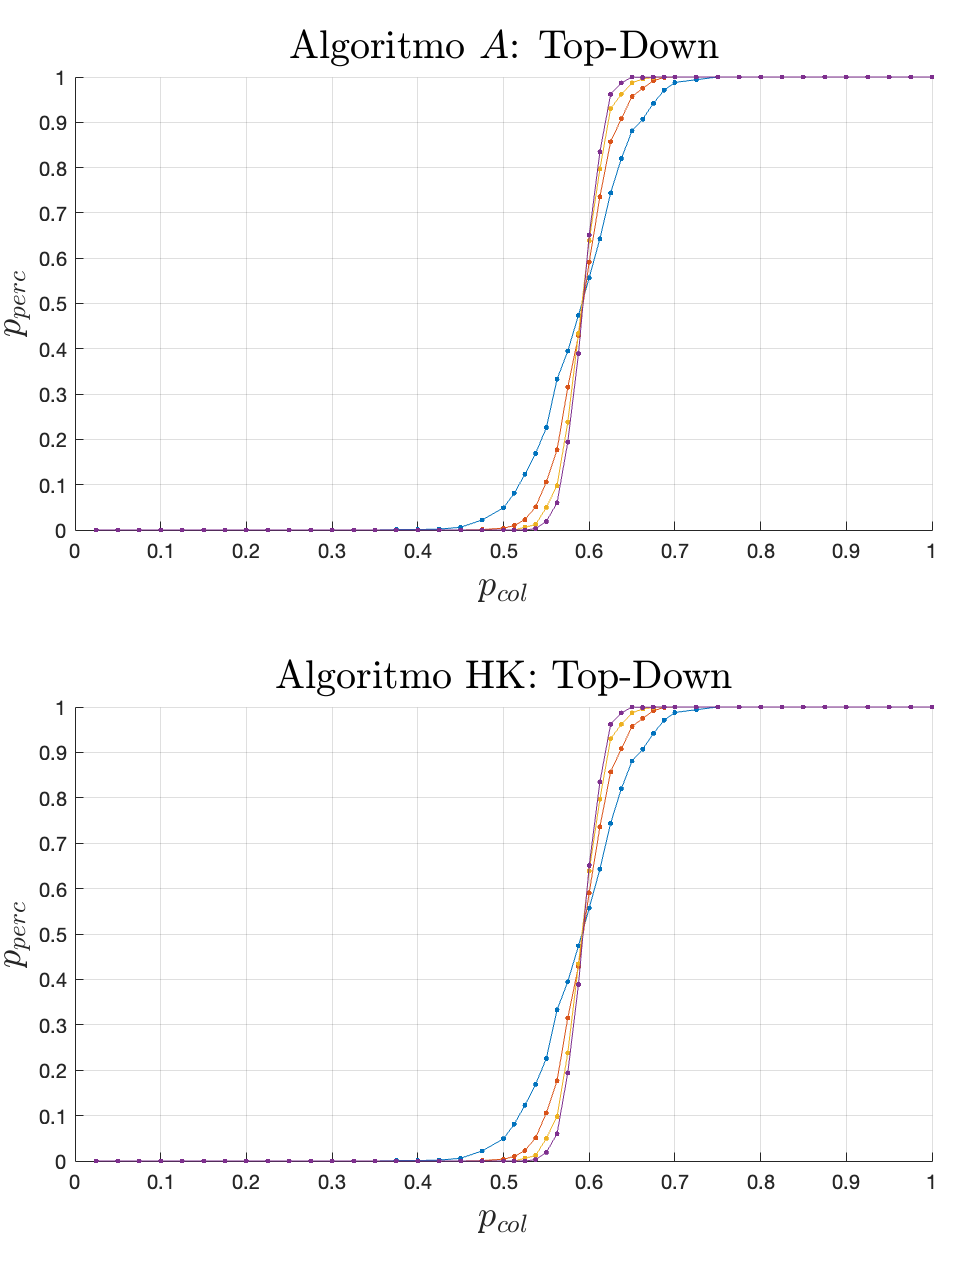
\includegraphics[width=0.9\columnwidth]{compare_threshold_1.png}
    \caption{Confronto tra le frequenze di percolazione top-down ottenute nell'esecuzione
    dei due algoritmi.}
    \label{fig:compare_threshold}
\end{figure}
Risulta interessante eseguire un confronto con la Fig. \ref{fig:threshold} 
relativa al reticolo di taglia infinita: per dimensioni del reticolo più grandi, ci 
si avvicina infatti al suddetto grafico.
Un'altra caratteristica importante da verificare è che le frequenze di 
percolazione top-down registrate coincidano con quelle left-right, nel limite 
dell'errore commesso. Le modalità di svolgimento sono le stesse, con l'aggiunta 
delle misurazioni dell'errore, calcolato come radice quadrata della quantità 
$D_{f_{perc}}$ descritta nell'Eq. \ref{eq:d_f_perc}.
Nel grafico in Fig. \ref{fig:th_errors} viene mostrato un confronto tra i valori 
ottenuti nei due casi con l'algoritmo HK. Ciò che balza all'occhio è la 
superiorità degli errori intorno a $0.6$, valore in cui, tra l'altro, 
si osserva una crescita piuttosto rapida della frequenza di percolazione.
Si compone di 3 iterazioni: una per variare la 
taglia del reticolo, una per variare la probabilità di occupazione e un'ultima per 
eseguire un numero sufficiente di esperimenti perché i risultati siano significativi.
Le frequenze dei due algoritmi sono calcolate con metodi diversi ma equivalenti:
nel primo caso si ``conta'' quante volte la variabile caratteristica ha assunto valore 1
e si divide il totale per il numero di esperimenti $N$; nel secondo caso si utilizza la 
funzione built-in di Matlab \texttt{mean(x)}, che svolge gli stessi passaggi.
Il Cod. \ref{cod:compare} mostra le istruzioni in Matlab per calcolare le quantità 
mostrate nei due grafici. Si è omessa l'implementazione in codice Matlab delle funzioni 
\texttt{CercaCluster3} e \texttt{CercaClusterHK}, del tutto analoghe all'implementazione 
mostrata tramite pseudocodice nei Cod. \ref{alg:standard} e \ref{alg:HK}. \\


\begin{figure}[ht]
    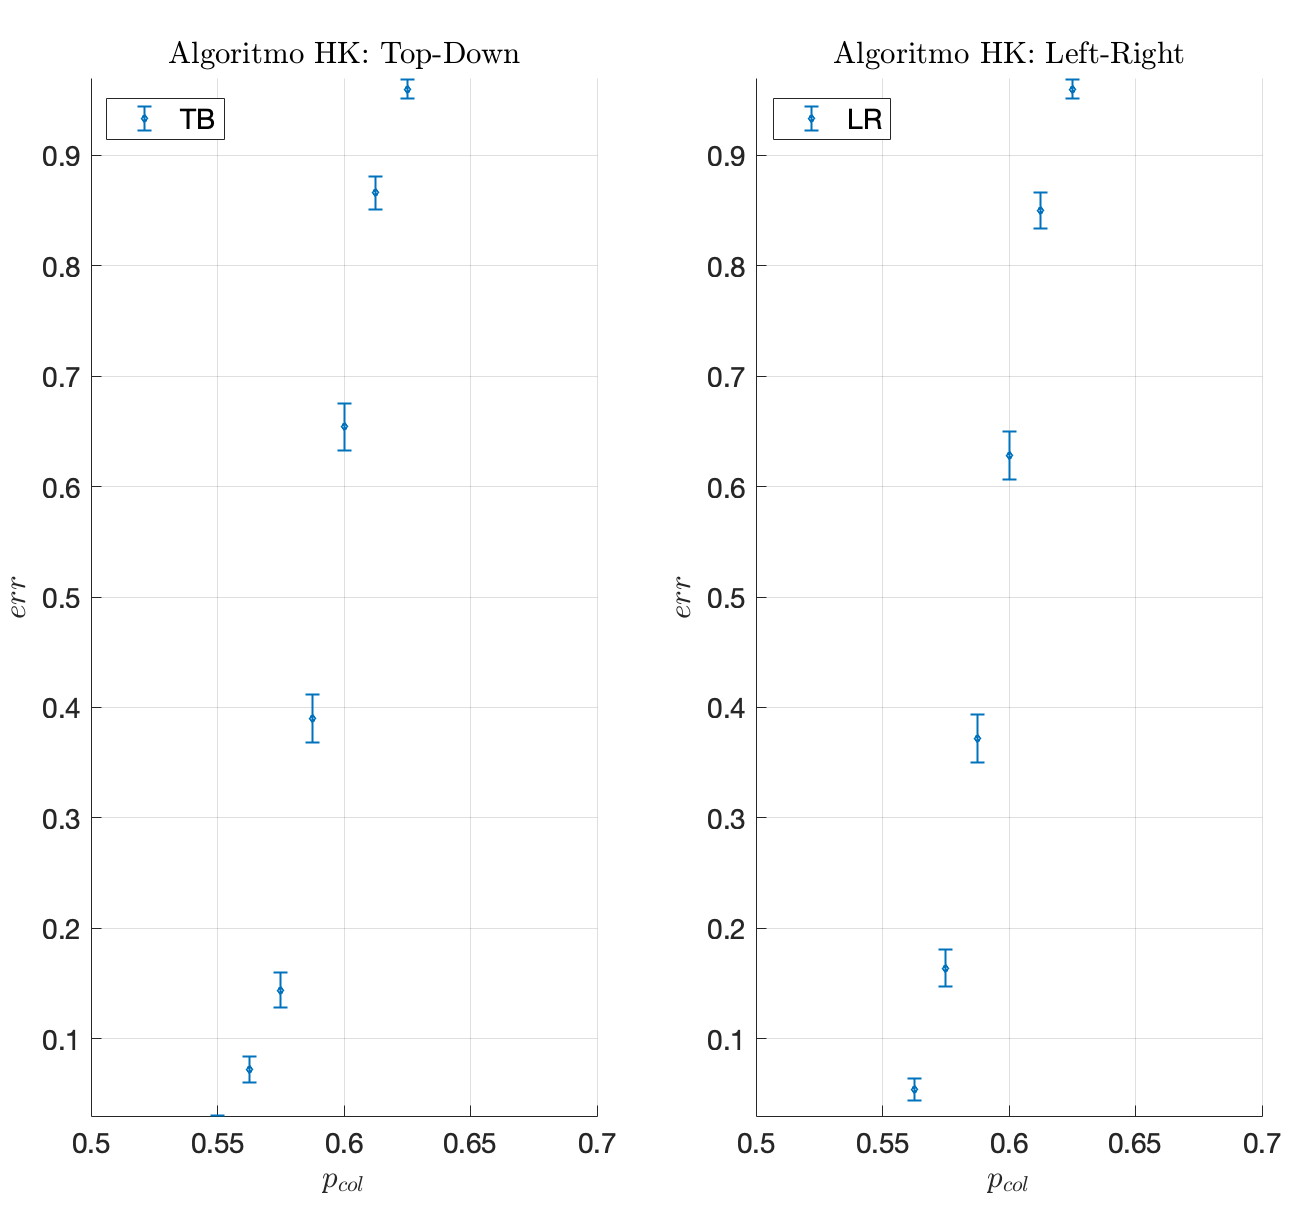
\includegraphics[width=\columnwidth]{errors.png}
    \caption{Confronto tra le frequenze di percolazione top-down e left-right,
    con rispettivi errori.}
    \label{fig:th_errors}
\end{figure}
\begin{lstlisting}[caption={Porzione di codice relativa al confronto tra algoritmi e 
    alla frequenza di percolazione top-down e left-right.}, label={cod:compare}]
for ij = 1:length(L)
    for ii = 1:length(p)
        pp = p(ii);
        s3TB = 0;
        s3LR = 0;
        sHKTB = 0;
        sHKLR = 0;
        espTB = zeros(N,1);
        espLR = zeros(N,1);
        for j = 1:N
            ret = rand(L(ij))<pp;
            res3 = CercaCluster3(ret);
            resHK = CercaClusterHK(ret);

            s3TB = s3TB + res3.percolazioneTB;
            s3LR = s3LR + res3.percolazioneLR;
            espTB(j) = resHK.percolazioneTB;
            espLR(j) = resHK.percolazioneLR;
        end

        probPercTB3(ij,ii) = s3TB / N;
        probPercLR3(ij,ii) = s3LR / N;
        probPercTBHK(ij,ii) = mean(espTB);
        probPercLRHK(ij,ii) = mean(espLR);
        erroreTB(ij,ii) = std(espTB) / sqrt(N);
        erroreLR(ij,ii) = std(espLR) / sqrt(N);
    end
end
\end{lstlisting}

\subsection*{Calcolo delle osservabili}
Lo stesso procedimento necessario per calcolare la frequenza di percolazione è stato svolto per 
le altre osservabili. In Fig. \ref{fig:distributions} si possono riscontrare i comportamenti 
attesi, descritti nella sezione precedente.
Anche in questo caso, viene acclusa l'implementazione in Matlab nel Cod. \ref{cod:distributions}.
Insieme alle quantità, vengono calcolati anche i rispettivi errori, con tecniche analoghe a quanto visto 
fin ora. Per queste quantità valgono le stesse considerazioni fatte sulla natura di $f_{perc}$,
legate alla validità della media e varianza garantita per mezzo di 
TLC e Legge dei Grandi Numeri.
\begin{figure}[ht]
    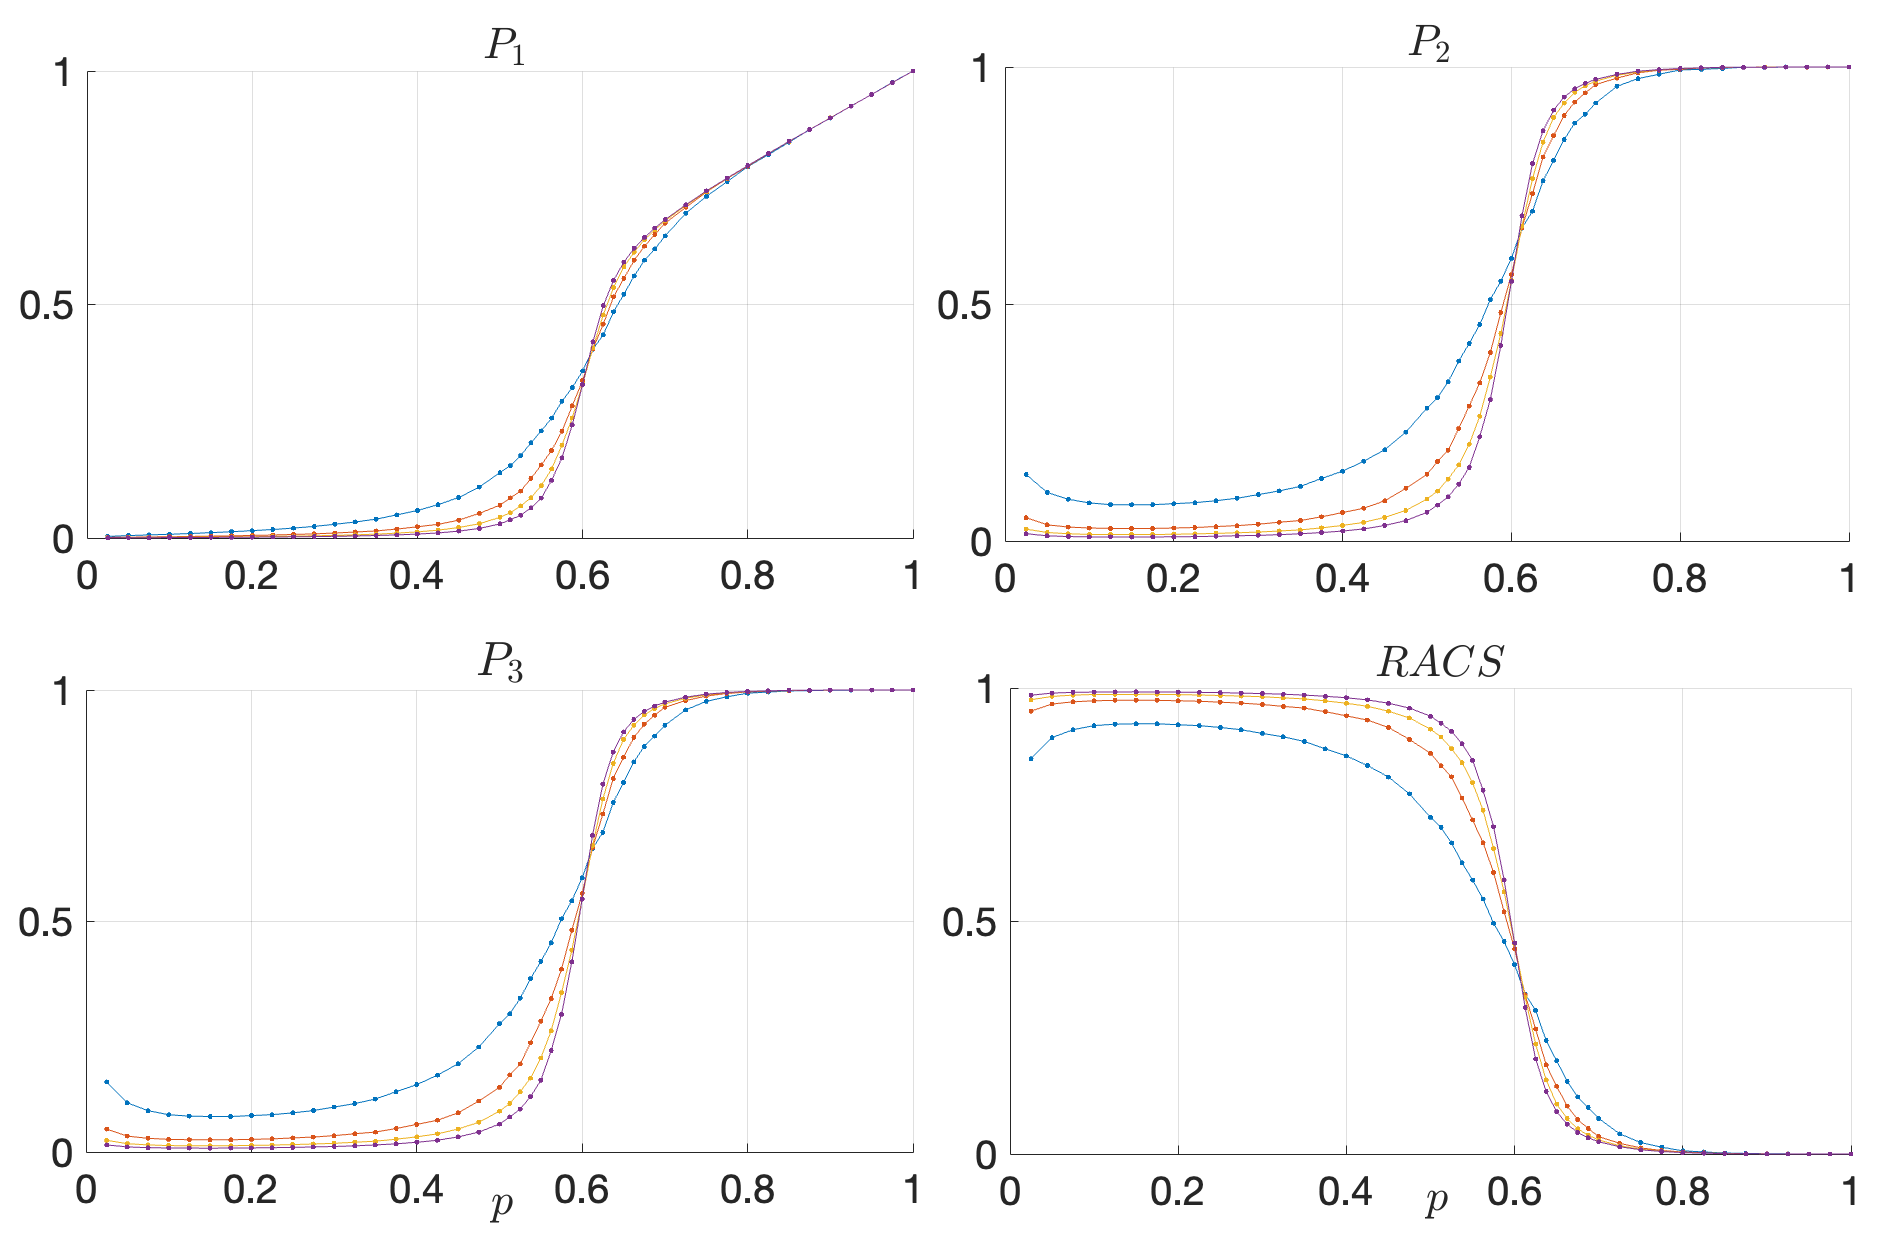
\includegraphics[width=\columnwidth]{p1p2p3racs_3.png}
    \caption{Distribuzioni delle osservabili calcolate in $N=1000$ esperimenti al variare dei parametri.}
    \label{fig:distributions}
\end{figure}
\begin{lstlisting}[caption={Porzione di codice per il calcolo delle osservabili.},label={cod:distributions}]
for ij = 1:length(L)
    for ii = 1:length(p)
        pp = p(ii);
        for j = 1:N
            ret = rand(L(ij))<pp;
            resHK = CercaClusterHK(ret);

            MYsz(ij,j,ii) = mean(resHK.cluSz);
            MYmaxSz(ij,j,ii) = max(resHK.cluSz);
            MYnumCLU(ij,j,ii) = length(resHK.cluSz);
            MYnumCol(ij,j,ii) = sum(resHK.cluSz);
        end
    end
   
    sMax=squeeze(MYmaxSz(ij,:,:));
    P1=sMax./L(ij)^2;
    errore1=std(P1)./sqrt(length(P1));
    P1=mean(P1);

    P2=sMax./(p*L(ij)^2);
    errore2=std(P2)./sqrt(length(P2));
    P2=mean(P2);

    occupied=squeeze(MYnumCol(ij,:,:));
    P3=sMax./occupied;
    P3=squeeze(P3);
    errore3=std(P3)./sqrt(size(P3,2));
    P3=mean(P3);

    occupiedReduced = squeeze(MYnumCol(ij,:,:)-MYmaxSz(ij,:,:));
    racs=occupiedReduced./occupied;
    erroreRacs=std(racs)/sqrt(length(racs));
    racs=mean(racs);
end
\end{lstlisting}

Per completezza, si aggiunge anche il grafico in Fig. \ref{fig:dist_errors} che confronta i vari errori 
ottenuti nel calcolo di ciascuna osservabile. Occorre prestare attenzione alla scala
sugli assi dei grafici: per questioni pratiche di visualizzazione, si è preferito
avere risultati più chiari, ma su scale leggermente diverse.
\begin{figure}[ht]
    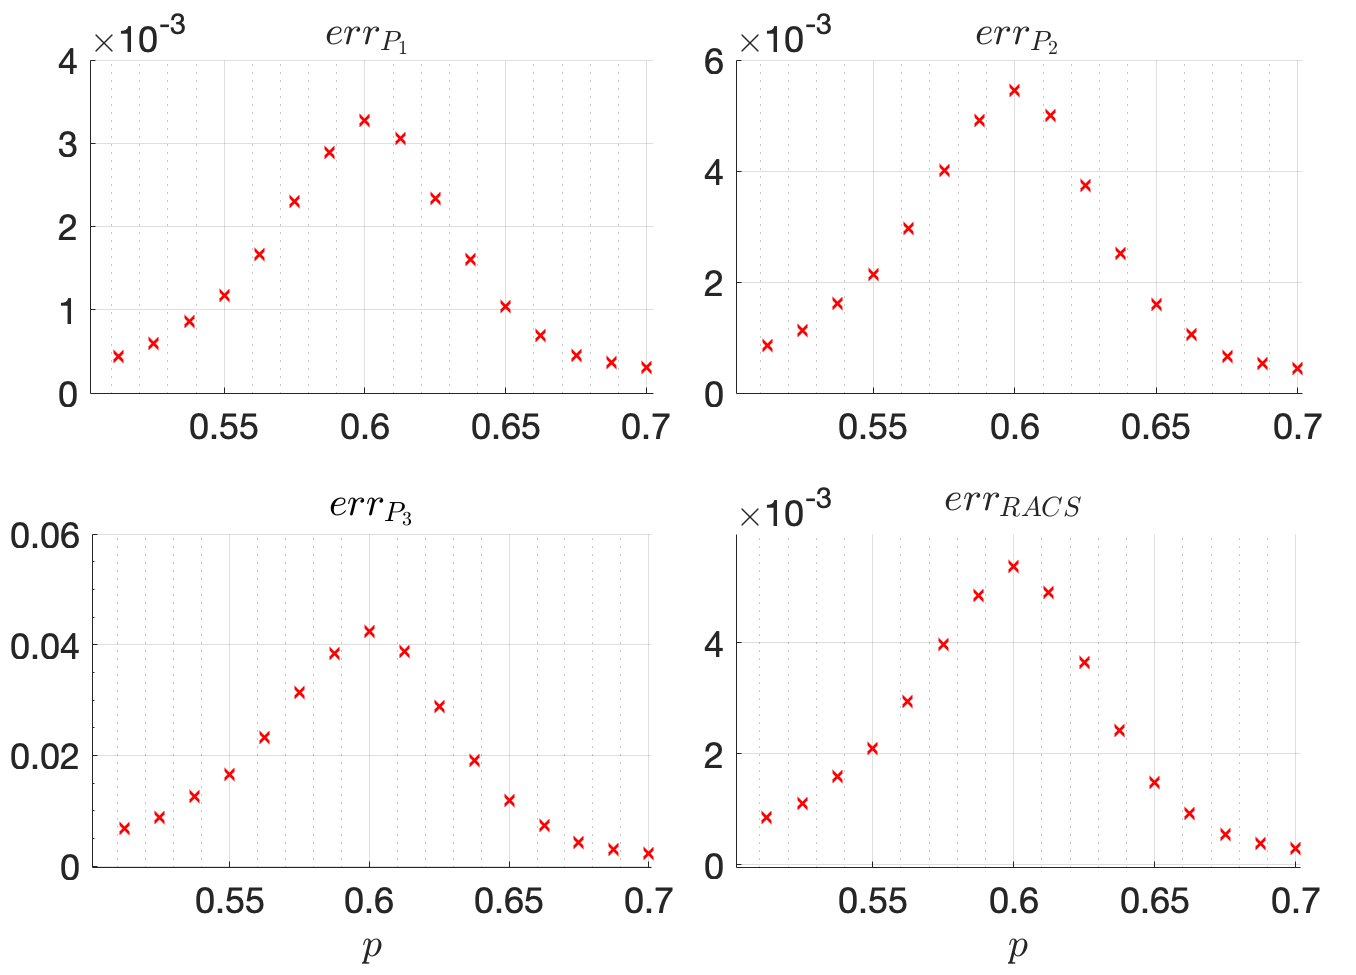
\includegraphics[width=\columnwidth]{dist_errors.png}
    \caption{Errori ottenuti nel calcolo delle osservabili.}
    \label{fig:dist_errors}
\end{figure}

\subsection*{Tempi di esecuzione}
Come ultimo risultato verranno discussi i tempi di esecuzione di ciascun algoritmo.
Prima di farlo, però, occorre precisare che Matlab non è l'ambiente di sviluppo migliore per valutare 
differenze di costo computazionale, a causa dei seguenti svantaggi (almeno per questo caso) che lo costituiscono:
\begin{itemize}
    \item operazioni matriciali: Matlab opera su strutture dati che rappresentano matrici,
        non è quindi ottimizzato per esecuzioni di tipo iterativo;
    \item ricorsione: le strutture dati utilizzate per 
        rappresentare il controllo di flusso non sempre sono adatte a sostenere lo spazio 
        richiesto da chiamate ricorsive;
    \item tic toc: il metodo per misurare i tempi di esecuzione non ha un buon funzionamento 
        in caso di quantità elevate di prove ripetute, soprattutto se molto vicine tra loro.
\end{itemize}
In fondo, Matlab rimane un linguaggio relativamente di alto livello rispetto 
ad alcune sue controparti come C++ per \texttt{opencv}.
Esistono alcune funzionalità che permettono di generare codice C++ o per GPU, ma non verranno affrontate in questa relazione.
Va comunque ricordato che Matlab ha molti altri pregi, tra cui la flessibilità
per la creazione di modelli, caratteristica fondamentale per il progetto.
Per tutte queste ragioni, i due algoritmi sono stati confrontati solo sulla parte 
relativa al cluster-finding. Il motivo dietro a questo è che nell'algoritmo Hoshen-Kopelman sono 
necessarie chiamate ricorsive per capire se due siti appartengono allo stesso cluster, e questa 
proprietà va verificata per tutti i siti dei bordi, causando un \textit{overhead}.
\begin{figure}[ht]
    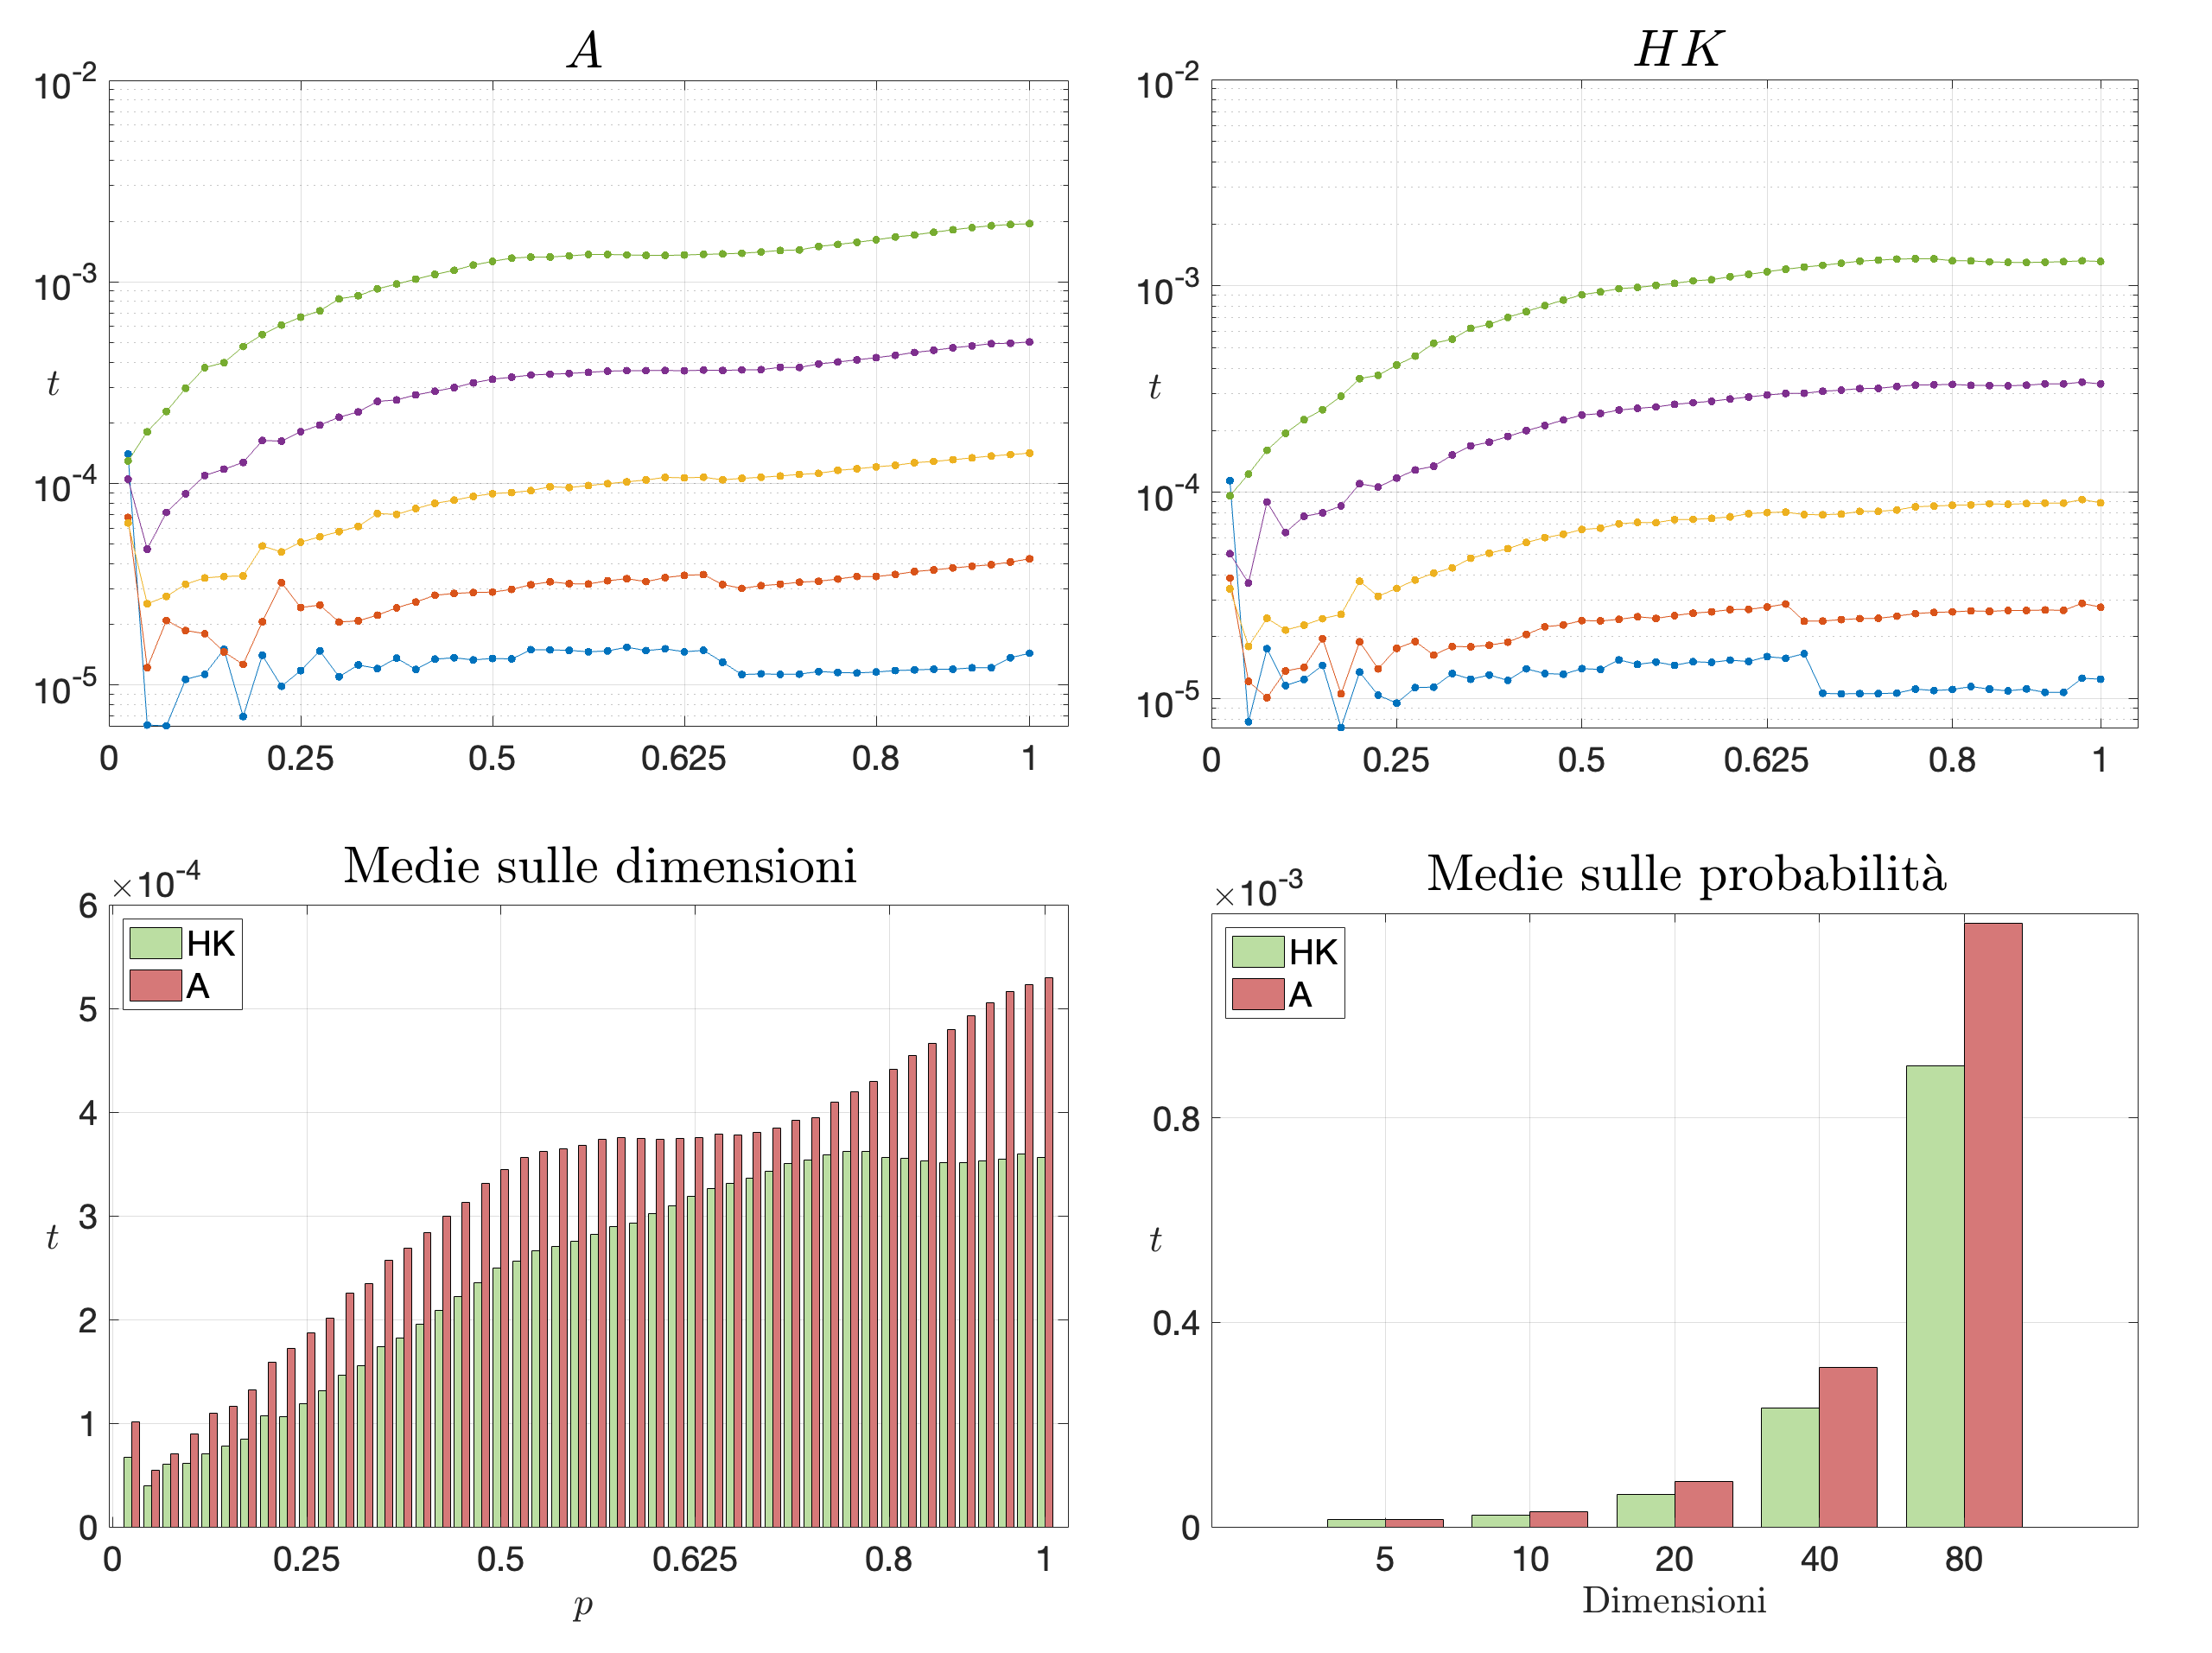
\includegraphics[width=\columnwidth]{times.png}
    \caption{Confronto dei tempi di esecuzione dei due algoritmi.}
    \label{fig:times}
\end{figure}

In Fig. \ref{fig:times} sono presenti 4 grafici che mostrano un confronto sugli andamenti dei 
tempi di esecuzione calcolati nelle due casistiche.
Anche in questo caso, la statistica viene fatta fissando i parametri (dimensione e probabilità di occupazione),
per poi effettuare un numero $N$ arbitrariamente grande di esperimenti.
Viene quindi eseguito prima $N$ volte l'algoritmo $A$, registrando il tempo impiegato e dividendolo per $N$
(si ottiene quindi una media per l'esecuzione singola).
Lo stesso viene fatto per l'algoritmo $HK$. Ciò che si ottiene sono due matrici $|P| \times |D|$, 
dove $D=[5 \; 10 \; 20 \; 30 \; 40]$ è l'array delle dimensioni e $P$ è l'array delle probabilità di 
occupazione.

I primi due grafici rappresentano proprio le due matrici ottenute, dove gli assi $y$ sono in scala 
logaritmica per avere un confronto visivo migliore. I diversi colori indicano le dimensioni dei reticoli 
degli esperimenti. Anche se di poco, in generale si notano tempi minori nell'algoritmo $HK$.
Nel terzo grafico viene fatta una media sulle dimensioni, in modo che rimangano solo due serie di dati da confrontare.
In pratica, si può pensare alle quantità mostrate nel terzo grafico come ``medie'' di quelle mostrate nei primi due.
Nell'ultimo caso, invece, la media viene fatta sulle probabilità e la lunghezza delle serie di dati da confrontare è 
5, come il numero di dimensioni. Anche in questo caso, le tempistiche di $HK$ sono minori rispetto ad $A$, come 
si aveva ragione di credere.
% \section{Conclusioni}

In conclusione, il progetto ha permesso di analizzare 
il fenomeno della percolazione attraverso un approccio frequentista, 
utilizzando due diversi algoritmi: uno standard $A$ e l'algoritmo di Hoshen-Kopelman. 
L'analisi statistica sui risultati ottenuti ha fornito una visione chiara dei 
meccanismi di percolazione e delle differenze di efficienza tra i due 
metodi implementati. Un naturale sviluppo futuro potrebbe essere lo studio 
del fenomeno su reticoli di forme diverse o in dimensioni superiori, come 
il caso tridimensionale, per esplorare eventuali variazioni nei comportamenti
osservati. Inoltre, un'interessante prospettiva di miglioramento sarebbe 
l'integrazione del codice Matlab con C++ tramite gli strumenti dedicati, 
permettendo una maggiore ottimizzazione delle strutture dati e 
un incremento dell’efficienza computazionale.

\bibliographystyle{IEEEtran}
\bibliography{main}

\end{document}
